%\documentclass[aps,prb,superscriptaddress,showpacs,reprint]{revtex4-1}
\documentclass[3p,twocolumn]{elsarticle}
\usepackage{fullpage}
\usepackage{amsfonts}
\usepackage{amssymb}
\usepackage{amsmath}
\usepackage{hyperref}
\usepackage{graphicx}% Include figure files
\usepackage{epstopdf}
\usepackage{subfig}
\usepackage[normalem]{ulem}
\begin{document}
%\usepackage{setspace}\doublespace
\title{ BCS-pairing versus ``moth-eaten effect'' in BEC-BCS crossover}
\author[uiuc]{Guojun Zhu\corref{cor1}}
%\affiliation{Department of Physics, University of Illinois at Urbana-Champaign, 1110 W Green St, Urbana, IL, 61801}
\ead{gzhu1@illinois.edu}
\author[uiuc,upmc]{Monique Combescot}
\ead{Monique.Combescot@insp.jussieu.fr}
%\affiliation{Institut des NanoSciences de Paris, Universite Pierre et Marie Curie, CNRS, Tour 22, 4 place Jussieu, 75005 Paris }
%\affiliation{Department of Physics, University of Illinois at Urbana-Champaign, 1110 W Green St, Urbana, IL, 61801}

%\affiliation{Department of Physics, University of Illinois at Urbana-Champaign, 1110 W Green St, Urbana, IL, 61801}
\address[uiuc]{Department of Physics, University of Illinois at Urbana-Champaign, 1110 W Green St, Urbana, IL, 61801}

\address[upmc]{Institut des NanoSciences de Paris, Universite Pierre et Marie Curie, CNRS, Tour 22, 4 place Jussieu, 75005 Paris }
%\cortext[cor1]{+1-217-3335224}
\newcommand{\vk}{\ensuremath{\mathbf{k}}}
\providecommand{\vr}{\ensuremath{\mathbf{r}}}
\newcommand{\vp}{\ensuremath{\mathbf{p}}}


\providecommand{\comm}[1]{\textit{\scriptsize \uwave{(#1)}}}
\newcommand{\td}{{\ensuremath{{\text{(2D)}}}}}
\newcommand{\sd}{{\ensuremath{{\text{(3D)}}}}}
\newcommand{\Arctg}{\ensuremath{\text{Arctg}}}



\numberwithin{equation}{section}
\begin{abstract}
We study the condensation energy change from a single bosonic pair of fermionic atoms to a large amount of pairs interacting via the reduced BCS potential. We find that the energy-saving due to correlations decreases when the pair number increases because the number of empty states available for pairing gets smaller ("moth-eaten effect"). However, this decrease is smaller at first than the 3D kinetic energy increase of the same amount of noninteracting atoms; it only dominates  when the total number of pairs approaches a fraction of the number of states available for pairing. As a result, the condensation energy per pair first increases and then decreases with pair number while in 2D, it always decreases.  
\end{abstract}
\begin{keyword}
A.Superconductor; D.Cooper Paring; D.Crossover
\end{keyword}

\maketitle
\section{Introduction}
It was known for a long time that a 3D system having a weak attractive potential cannot sustain a bound-state.  In 1956, Cooper showed that in the presence of a frozen Fermi sea, a pair of electrons with opposite spin can form a bound-state of zero total momentum  no matter how weak the attraction is\cite{Cooper}.  This state actually is indeed a many-body state because the  Fermi sea, even if it does not interact through the reduced BCS potential,  is essential for the formation of ``two-body'' bound state.   The next year, Bardeen, Cooper and Schrieffer introduced a many-body ansatz which is an extension of this single pair ``bound state'' and showed that this ansatz gives an intricate many-body state with lower energy than free Fermi gas with arbitrarily weak attraction\cite{BCS} for the same reduced BCS hamiltonian.  They used a particle-number non-conserved ansatz in a grand-canonical ensemble.  Nevertheless, the reduced BCS model also has a frozen Fermi sea in the core.
  Later,   Gor'kov and Melik-Barkhudarov showed that the frozen Fermi sea is not necessary and the same idea works with a renormalized attraction measured by low energy scattering amplitude\cite{Gorkov}.   Furthermore, Eagles\cite{Eagle}, Leggett\cite{LeggettCrossover}, Nozi\`{e}res and Schmitt-Rink\cite{Nozieres} extended the BCS pairing idea and bridged Cooper pairing and molecular BEC. There they used the model without a frozen Fermi sea as core and employed the full k-space.  All these lead to an interesting question that how the solution for the same hamiltonian evolves from one-pair, where there might be no bound state, to infinite number of pairs, where a many-body bound solution always exists.  Nevertheless, the particle non-conserved nature of the BCS ansatz makes it inherently many-body, which is quite difficult to connect to one-pair solution.  

Five years after BCS, Richardson showed that a number-conserved eigenstate exists for the reduced BCS Hamiltonian and it gives the same energy as BCS ansatz in thermodynamic limit\cite{Richardson1,Richardson2,Richardson3,Richardson1968,gaudin}.  In the model, a frozen Fermi sea also exists in order to provide a constant density of states.  Since 2000, we developed a new theoretical framework for composite bosons (cobosons for short) formed by fermion pairs for electron excitons\cite{CobosonPhysicsReports}.   Recently, we applied it into superconductivity and it was proved to be useful.  We rederived Richardson-Gaudin equations with coboson framework\cite{CobosonBcsRich}. We also studied Richardson equations in details \cite{CombescotCooper,combescotBCS}.  Richardson-Gaudin solution, as a number-conserved one, is  particular suitable to investigate the question we raised.  

It is illuminating to image the additional pair was added to the system of few tightly-bound pairs.   Pauli exclusion would show in two different places roughly speaking.  (i) Pairing (binding) happens in more restricted phase space, and therefore the energy saving by potential becomes less than the previous pair, which enjoy larger phase space.  This is the moth-eaten effect we discussed in exciton context extensively\cite{CobosonPhysicsReports}.  (ii) On the other hand, in free fermion gas where there is no attraction, the extra fermions has to piled in the next k-level and also cost more energy due to Pauli exclusion.  Of course, these two effects must be solved in a self-consistent fashion.  We will do that in sec. \ref{sec:twoPair}.  Nevertheless, it is useful to separate them in order to build some intuition on the problem.  In a 3D system with strong attraction, we can estimate the first effects from our previous work in exciton, the energy decrease is in order of $N\frac{a^3}{V}$, where $N$ is the total number of pairs, $a$ is the average size of pair in two-body Schr\"{o}ndinger equation, and $V$ is the volume of the system. The second effect is in order $1/\rho(\epsilon_F)$, where $\rho(\epsilon)\sim\sqrt{\epsilon}$ is the density of the state, $\epsilon_F\sim\left(\frac{N}{V}\right)^{2/3}$. So the new pair would cost energy in ordr of $\left(\frac{V}{N}\right)^{2/3}$. When $N$ is small, (ii) dominates (i). Therefore, the condensation energy, the difference between the system energy with potential and without potential (as free gas), increases.  And when $N$ gets larger and larger, (ii) increases not as fast as (i) and finally (i) dominates and condensation energy decreases.    This argument is somewhat hand-waving, yet the intuition here proves to be quite close to truth.  We will set them in solid ground in the following parts of the paper. 

We illustrate our model in sec. \ref{sec:model}.  In sec. \ref{sec:onePair}, we study the one-pair problems in detail for both 2D and 3D.  We discussed the N-pairs problems, and make some conjecture about their connection with one-pair solution  in sec. \ref{sec:NPair}.  And we will attempt 2-pair Richardson-Gaudin equations and put the conjecture into the solid ground in sec \ref{sec:twoPair}.  And we will offer some final thought in sec. \ref{sec:conclusion}.

\section{Physical understanding}
\subsection{The model\label{sec:model}}
We consider $N$ fermionic atoms with creation operators $a_\vk^\dagger$ and $b_\vk^\dagger$  governed by the hamiltonian
$H=H_{0}+V$. The kinetic part $H_0$ reads as 
\begin{equation}
H_0=\sum_{\vk}\epsilon_\vk(a^\dagger_\vk{}a^{}_\vk+b^\dagger_\vk{}b^{}_\vk)
\label{eq:}
\end{equation}
We take as $V$ the reduced BCS potential without its usual frozen core, namely
\begin{equation}
V=-v\sum_{\vk\vk'}w_{\vk'}w_\vk\beta^\dagger_{\vk'}{}\beta^{}_\vk
\label{eq:VBcs}
\end{equation}
 where $\beta^\dagger_{\vk}=a^\dagger_{\vk}b^\dagger_{-\vk}$ while $w_\vk=1$ for $0<\epsilon_\vk<\Omega$ and zero otherwise, so that attraction acts from zero to a sharp cutoff $\Omega$. This cut-off bears no connection with phonon energies but can be related to the scattering length, as shown below.
 \subsection{One pair\label{sec:onePair}}
The single pair energy $E_1$ in this potential follows from Cooper's equation
\begin{equation}
1=v\sum_{\vk}\frac{\omega_\vk}{2\epsilon_\vk-E_1}\equiv{}v\,S(E_1)
\label{eq:onePair}
\end{equation}

(i) In 2D, the density of state is constant, so that for negative $E$, 
\begin{equation}
S^{(\text{2D})}(E<0)=\rho\int_0^{\Omega}\frac{d\epsilon}{2\epsilon-E}=\frac{\rho}{2}\ln\left(\frac{2\Omega-E}{-E}\right)
\label{eq:s1pair}
\end{equation}
%\begin{figure}[htbp]
	%\centering
		%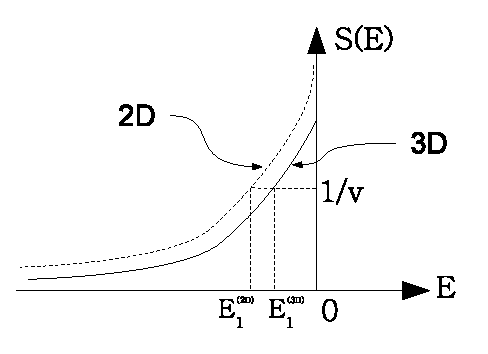
\includegraphics[width=0.30\textwidth]{OnePair.eps}
	%\caption{The functions $S(E)$ in 2D and 3D.}
	%\label{fig:OnePair}
%\end{figure}
goes to infinity when $E\rightarrow{}0_{-}$ while it goes to zero as $\rho\Omega/(-E)$ when $E\rightarrow-\infty$. A bound state with $E_1<0$, solution of Eq. (\ref{eq:onePair}), thus exists no matter how weak $v$ is. It reads
$
E_1^{(\text{2D})}=-\frac{2\sigma}{1-\sigma}\Omega
$
with $\sigma=e^{-2/\rho{v}}$. Note that while $\rho$ increases linearly with sample volume, $\rho{v}$ stays constant.

(ii) In 3D, the density of states reads as  
$\rho(\epsilon)=\rho\sqrt{\epsilon/\Omega}$
where $\rho$ now is the density of state at the potential upper boundary. We then find that
\begin{equation}
\begin{split}
S^\sd(E<0)&=\rho\int_0^{\Omega}{}d\epsilon\frac{\sqrt{\epsilon/\Omega}}{2\epsilon-E}\\
	&=\rho(1-\sqrt{\frac{-E}{2\Omega}}\Arctg\sqrt{\frac{2\Omega}{-E}})
\label{eq:}
\end{split}
\end{equation}
goes to $\rho$ when $E\rightarrow0_-$ while it goes to zero as $\frac{2}{3}\rho\Omega/(-E)$ when $E\rightarrow-\infty$. 
A bound state with $E_1<0$ thus exists for $v$ larger than a threshold value $v_{\text{th}}(N=1)=1/\rho$.  For a potential just above threshold, the single pair energy in 3D tends to zero as 
$
E_1^\sd\approx-8(\rho v-1)^2\Omega/\pi^2
$
while far above threshold
$E_1^\sd\approx-\frac{2}{3}\rho{v}\Omega$

(iii) We can use this result to relate the s-wave scattering length $a_{s}$ to the potential threshold $\Omega$ via the density of state $\rho$ at the upper boundary. Indeed, for fermion pairs interacting via the bare potential $v^{0}_{\vk'\vk}=-v \omega_{\vk'}\omega_\vk$, the s-wave T-matrix reduces to
\begin{equation}
T^{0}_{k}=\frac{-v\omega_k}{1-vS(2\epsilon_k+i0_+)}
\end{equation}
with $S^\sd(2\epsilon_k+i0_+)\simeq\rho(1+i\pi\sqrt{\epsilon_k/4\Omega})$  for $\epsilon_k\ll\Omega$. We then get the scattering length through the scattering amplitude $f^0_k= -a_s/(1+ika_s)$ which depends on the T-matrix as $f^0_k= -mL^3T^{0}_{k}/4\pi$ for a sample volume $L^3$. This gives $a_s\propto -v/(1-\rho v)$. For $v$ slightly below the $1/\rho $ threshold, $a_s$ is positive, the pair binding energy reading $E_{b}\approx-1/(ma_s^{2})$ while below threshold, $a_s$ is negative and no bound state exists. 

\subsection{N pairs\label{sec:NPair}}
Richardson \cite{Richardson1} and Gaudin \cite{gaudin} have shown that the energy of $N$ fermion pairs interacting through the reduced BCS potential reads $E_N=R_1+\cdots+R_N$ where the $R_i$'s follow from $N$ equations
\begin{equation}
 1=v\sum_\vk\frac{w_\vk}{2\epsilon_\vk-R_i}+\sum_{j\neq{}i}\frac{2v}{R_i-R_j}
\end{equation}

-- {\it 2D systems}: Very recently(refs..), we have derived a compact expression for the $N$-Cooper pair energy in standard BCS superconductivity, with a constant density of state above a 3D frozen core. Using this result for 2D systems which also have a constant density of states, we find
\begin{equation}\label{eq:E2dN}
 E^\td_N=N\,E^\td_1+\frac{N(N-1)}{\rho}\frac{1+\sigma}{1-\sigma}
\end{equation}
within underextensive terms $(N/\rho)^n$ with $n\geqslant2$.
If we now consider energies without and with potential
$
E_N^{\td}(v=0)-E_N^\td= 
%\mathcal{E}^{(2D)}_N
\Delta E^{(2D)}_N
$,
Eq.(\ref{eq:E2dN}) gives the condensation energy per pair $\epsilon_N^\td = \Delta E^{(2D)}_N/N$ as
  \begin{equation}
\epsilon^{(2D)}_N=(1-\frac{N-1}{N_\Omega})\frac{2\sigma}{1-\sigma}\Omega\label{eq:E2D}
\end{equation}
where for 2D, the total number of states in the potential layer is $N_\Omega=\sum_k{}w_{\vk}=\rho\Omega$. This shows that $\epsilon^\td_N$  decreases linearly with $N$. This decrease is due to a moth-eaten effect induced by Pauli blocking on the number empty states feeling the potential and thus available to form the correlated $N$-pair state.  At complete filling, we find $
 \epsilon^\td_{N_\Omega}=[\frac{2\sigma}{1-\sigma}]\Omega/\rho
$
so that $
 \epsilon^\td$ goes to zero as $1/\rho$ in the large sample limit: for $N=N_\Omega$, the system has  essentially lost all its freedom to construct a lower energy state.


%\begin{figure}[htbp]
	%\centering
		%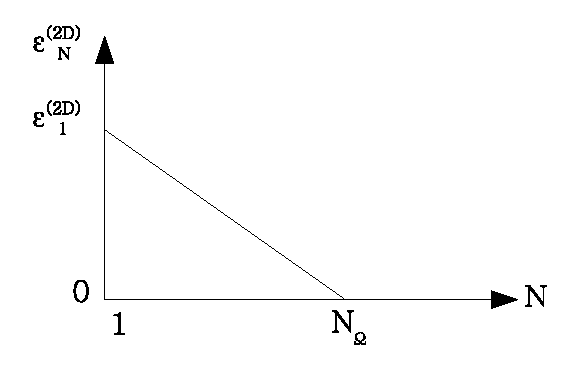
\includegraphics[width=0.30\textwidth]{2dCondEnergy.eps}
	%\caption{Condensation energy per pair as a function of the pair number in 2D systems.}
	%$N_{\Omega}=\rho\Omega$ is the total number of pair state in the potential layer
	%\label{fig:2dCondEnergy}
%\end{figure}




-- {\it 3D systems}: A  similar compact expression of the $N$-pair energy does not exist for a $\sqrt{\epsilon}$ density of states. We are thus mostly left with qualitative understanding. 

(i) First, due to the same lack of available states, the moth-eaten effect must bring the condensation energy per pair down to zero when $N$ approaches the total number of pairs in the potential layer, which in 3D reads as $N_\Omega=\sum_{\vk}w_{\vk}=\frac{2}{3}\rho\Omega$. 

(ii)
For $v$ smaller than $v_{th}(1)=1/\rho$, the condensation energy per pair $\epsilon_N^\sd$ is equal to zero for $N=1$ and also for $N=N_\Omega$ due to the moth eaten effect.  It is however clear that $\epsilon_N^\sd$ cannot stay equal to zero for all $N$ because when $N$ approaches $N_\Omega$, we can always think of freezing $N_0$ of these electrons as in standard BCS superconductivity. The density of states for the remaining $N_\Omega - N_0$ states being essentially constant, a finite condensation energy must  appear no matter how weak $v$ is.  We can then use 
%\begin{figure}[htb]
	%\centering
		%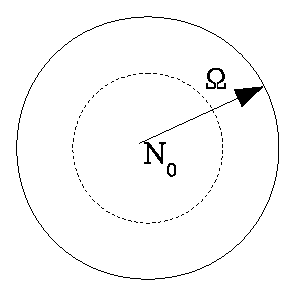
\includegraphics[width=0.20\textwidth]{potential.eps}
	%\caption{Effective frozen core in the case of many pairs in 3D system}
	%\label{fig:potential}
%\end{figure}
Eq. (\ref{eq:E2D}) to estimate it as
\begin{equation}\label{eq:E3D}
\Delta E_{N-N_0}=(N-N_0)(1-\frac{N-N_0-1}{N_\Omega})\frac{2\bar\sigma}{1-\bar\sigma}\Omega
\end{equation}
where $\bar{\sigma}=e^{-2/{\bar{\rho}v}}$ with $\bar\rho\simeq\rho$ being the average density of states above the frozen core. $\Delta E_{N-N_0}$ is maximum for $N-N_0=N_\Omega/2$.
This argument essentially shows that, even if $N$ is not as large as $N_\Omega/2$, but still a sizable faction of it,  a BCS-like collective effect  must take place to produce a non-zero condensation energy, no matter how weak $v$ is. 
As a result, the threshold potential  $v_{th}(N)$ for the appearance of a $N$-pair condensation  must decrease with $N$, down to essentially zero when $N$ is a sizable fraction of the total number of pairs $N_\Omega$ in the potential layer.  Consequently, for a given potential $v$, condensation starts at $N=N^*$ with $v=v_{th}(N^*)$. When $N$ increases above $N^*$, the condensation energy per pair first increases from zero and then return to zero (see Fig. \ref{fig:3dCondChange}), due to the moth-eaten effect which always dominates when most of the pair states available to form the condensate are occupied. 


%\begin{figure}[htb]
	%\centering
		%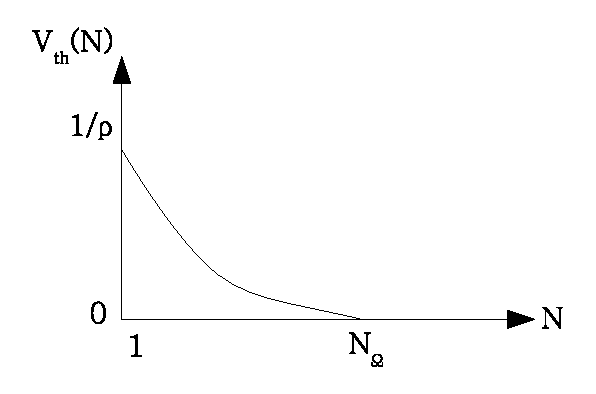
\includegraphics[width=0.30\textwidth]{3dThresholdChange.eps}
	%\caption{Threshold change against number of pairs in 3D}
	%\label{fig:3dThresholdChange}
%\end{figure}

(iii) For $v$ above threshold for single pair condensation, the condensation energy per pair $\epsilon^\sd_N$ is finite for $N=1$. We expect by continuity with the $v<v_{th}(1)$ case, that $\epsilon^\sd_N$ first increase with $N$ and then decreases due to the same moth-eaten effect which ends by controlling condensation when $N$ approaches full-filling.  
To physically understand this behavior, we must note that the condensation energy is the difference between two energies which both increase with $N$ due to Pauli blocking.  The question then is to understand why, for small $N$, the free pair energy increases faster than the correlated pair energy. When one free pair is added at the energy level $\epsilon$, the kinetic energy increases by $1/\rho(\epsilon)$.  In 3D systems with a density of states in $\sqrt{\epsilon}$, the free pair energy change when going from $N$ to $N+1$ pairs, is thus larger for low energy states. By contrast, correlated pairs are made with all pair states between $0$ and $\Omega$. When the pair number increases from $N$ to $N+1$, a very small fraction of each of these states is blocked, so that the energy change is far less than when blocking a single low energy state.  Consequently, when $N$ is small,  the energy difference between adding one free pair and one correlated pair must increase with $N$. W
 hen $N$ gets large, the cost in energy $1/\rho(\epsilon)$ to add one free pair stays essentially constant and equal to the cost to block any of the $\vk$ states making the correlated pair.  We are then left with the moth-eaten effect on the bound state itself which tends to decrease the condensation energy. 

Note that this understanding is fully supported by the monotoneous decrease of $\epsilon^\td_N$: Indeed, the 2D density of state is constant; so that the energy cost to block a single low energy state is the same as the one to block  any of the states making the correlated pair; so that we are left with the moth-eaten effect: the condensation energy per pair can only decrease when $N$ increases.  

In order to establish this qualitative understanding on stronger  grounds, let us consider $N=2$ pairs. This limiting case will give the trend of the $N$-dependence of $\epsilon^\td_N$ since it already contains the physics which drives this $N$-dependence, namely Pauli blocking.  

\begin{figure}[htb]
	\centering
		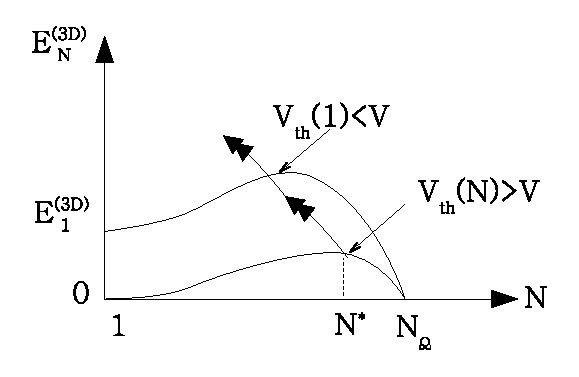
\includegraphics[width=0.8\columnwidth]{3dCondChange.eps}
	\caption{Condensation energy per pair as a function of pair number: in 2D, it always decreases due to the moth-eaten effect while in 3D, this effect dominates for large $N$ only.}
	\label{fig:3dCondChange}
\end{figure}

\section{Condensation energy for two pairs\label{sec:twoPair}}
The exact energy of two fermion pairs in the reduced BCS potential of Eq. (\ref{eq:VBcs}), reads $E_2=R_1+R_2$ where $(R_1,R_2)$ are solution of
\begin{equation}
1=v\sum_{\vk}\frac{w_\vk}{2\epsilon_\vk-R_1}+\frac{2v}{R_1-R_2}=(R_{1}\leftrightarrow{}R_{2})
\label{eq:richardsonEq}
\end{equation}
%By adding and substracting these two equations, and by using Eq.(\ref{eq:onePair}) for a single pair, we get
%\begin{gather}
%\begin{split}
%0=&(R_1-E_1)\sum_{\vk}\frac{w_\vk}{(2\epsilon_\vk-R_1)(2\epsilon_\vk-E_1)}\\
%&+(R_{1}\leftrightarrow{}R_{2})\label{eq:2PairPlus}
%\end{split}\\
%-\frac{4}{(R_1-R_2)^2}=\sum_{\vk}\frac{w_\vk}{(2\epsilon_\vk-R_1)(2\epsilon_\vk-R_2)}\label{eq:2PairMinus}
%\end{gather}
\subsection{2D systems}
We have solved these coupled equations analytically in the BCS case with a constant density of states above a frozen core\cite{combescotBCS}.  Using  this work  for 2D systems with a constant density of states for $0<\epsilon_k<\Omega$, we get the energy difference between two correlated pairs and two single pairs in the large sample limit, as 
\begin{equation}
E^{\td}_2-2E_1^{\td}=\frac{2}{\rho}\left(1+\frac{2\sigma}{1-\sigma}\right)+\text{O}(\frac{1}{\rho^2})
\label{eq:}
\end{equation}
$2/\rho$ is the kinetic energy cost to go from 1 to 2 pairs when the density of state is constant while $[2/\rho][2\sigma/(1-\sigma)]$ is the change in binding energy of two pairs induced by the moth-eaten effect. 

This result, far easier to get than the one for arbitrary $N$ given in Eq.(\ref{eq:E2dN}), not only shows the trend induced by Pauli blocking on the $N$ correlated pair energy, but also allows to obtain this energy exactly through a rule of the thumb that we have learned valid for all exciton problems studied up to now - excitons being like paired electrons, composite bosons with a many-body physics driven by Pauli blocking.  This rule says that, in the thermodynamical limit, i.e., large volume but $N/\rho$ constant, the result for $N$ is the result in 2 multiplied by $N-1$.  In the present case, this gives the energy change \emph{per pair}, $[E^{\td}_N-NE^{\td}_1]/N$, as $[(N-1)/\rho](1+\sigma)/(1-\sigma)$ in agreement with
Eq.(\ref{eq:E2dN}).


\subsection{3D systems}

3.2.1-- {\it For potential above the $N=1$ threshold}, $v>1/\rho$, we have shown that a single pair has a well defined bound state with $E_1$  finite negative. Since the change between the two-pair energy $R_{1}+R_{2}$ and the energy of two single pairs  $2E_{1}$ can only come from Pauli blocking due to the very peculiar form of the reduced BCS potential, we expect $R_1+R_2\approx2E_1$, when $L^3\rightarrow\infty$, i.e., when $\rho\rightarrow\infty$. This leads us to expand the sum in Eq.(\ref{eq:richardsonEq}) in terms of $(R_{1}-E_{1})$.  Using Eq.(\ref{eq:onePair}) for the first order term, we get
\begin{equation}
0=\sum_{n=1}^{\infty}(R_{1}-E_{1})^{n}\sum_{\vk}\frac{w_\vk}{(2\epsilon_\vk-E_1)^{n+1}}+\frac{2v}{R_1-R_2}
\end{equation}
The sum over $\vk$ replaced by an integral with a density of state $\rho\sqrt{\epsilon/\Omega}$, gives
\begin{multline}
\sum_{\vk}\frac{w_\vk}{(2\epsilon_\vk-E_1)^{n+1}}=\\\frac{\rho}{(-E_{1})^{n}}\sqrt{\frac{-E_{1}}{2\Omega}}K_{n}(\frac{2\Omega}{-E_{1}})
\end{multline}
where $K_{n}(x)$, defined as
\begin{equation}
K_{n}(x)\equiv\int_{0}^{x}\frac{\sqrt{y}\;dy}{2(y+1)^{n+1}}
\end{equation}
goes to $K_{n}$ when $x$ goes to infinity, which is the physically relevant limit since the single pair binding energy is much smaller than the potential extension $\Omega$.
This leads us to rescale the $R_{i}$'s in terms of $E_{1}$ according to
$R_{i}=E_{1}(1-t_{i})\quad\text{for }i=(1,2)$. Richardson-Gaudin equations (\ref{eq:richardsonEq}) then take a dimensionless form
\begin{equation}
0=\sum_{n=1}^{\infty}t_{1}^{n}K_{n}+\frac{1}{\rho\Omega}\left(\frac{2\Omega}{-E_{1}}\right)^{3/2}\frac{1}{t_1-t_2}=(t_{1}\leftrightarrow{}t_{2})
\end{equation}
If we now add and subtract these two equations, we get
\begin{gather}
0=\sum_{n=1}^{\infty}(t_{1}^{n}+t_{2}^{n})K_{n}\label{eq:t2}\\
-\lambda^{2}=(t_{1}-t_{2})\sum_{n=1}^{\infty}(t_{1}^{n}-t_{2}^{n})K_{n}\label{eq:t1}
\end{gather}
where we have set $\lambda^2=(1/\rho\Omega)(2\Omega/-E_{1})^{3/2}$.
Two different regimes can then be distinguished.  

(i) For $\lambda^{2}$ small, we get from Eq.(\ref{eq:t1}) $(t_{1}-t_{2})^{2}\approx-\lambda^{2}/K_{1}$. By writing $t_{1}^{2}+t_{2}^{2}$ as $\left[(t_{1}+t_{2})^{2}+(t_{1}-t_{2})^{2}\right]/2$, we then find from Eq.(\ref{eq:t2}), $(t_{1}+t_{2})^{2}\approx\lambda^{2}K_{2}/2K_{1}^{2}$.  So that the dominant term of the two correlated pair energy in the large sample limit reads as 
\begin{equation}
E_{2}=R_{1}+R_{2}\approx2\left(E_{1}+\frac{1}{\rho}\sqrt{\frac{2\Omega}{-E_{1}}}\frac{K_{2}}{K_{1}^{2}}\right)
\end{equation}
$E_{2}$ thus increases with sample size as $1/\rho\sim1/L^{3}$.

To get the condensation energy change, we have to compare this increase with the one of two free pairs.  Due to Pauli blocking, the momentum of the second pair is $2\pi/L$, so that the kinetic energy increase scales as $1/L^{2}$.  In the large $L$ limit, it is thus larger than the one of two correlated pair. 
As a result, the condensation energy per pair, which is the energy difference without and with potential, increases from 1 to 2 pairs - in agreement with the continuity argument of section 2. 

(ii) The $\lambda^{2}>1$ regime is  reached for $E_{1}$ small, more precisely for $-E_{1}<\Omega^{1/3}/\rho^{2/3}\approx1/mL^{2}$.  In this regime, the single pair binding energy is thus smaller than the kinetic energy difference between the two lowest free states. It is then impossible to replace the discrete sum over $\vk$ by a integral through a continuous density of state.  So that the above procedure to get the 2-pair energy becomes invalid.  


3.2.2-- {\it At potential threshold}, $v=1/\rho$, the single pair binding energy cancels so that we cannot rescale the $R_i$'s in terms of $E_1$ as we have done above threshold. The above $\lambda^{2}>1$ regime leads us to guess that, as for $E_1$ small, the threshold behavior, associated to $E_1=0$, cannot be derived by replacing the sum over $\vk$ by an integral.

To show it, let us first substract the two Richardson-Gaudin equations, Eqs.(\ref{eq:richardsonEq}). We get
\begin{equation}
-\frac{4}{(R_1-R_2)^2}=\sum_{\vk}\frac{w_\vk}{(2\epsilon_\vk-R_1)(2\epsilon_\vk-R_2)}\label{eq:2PairMinus}
\end{equation}
By writting $R_1+R_2=E_2=2R$ and $R_1-R_2=2iR'$ with $R$ real but $R'$ a priori complex, the above equation gives 
\begin{equation}
\frac{1}{R'^2}=\sum_{\vk}\frac{w_\vk}{(2\epsilon_\vk-R)^2+R'^2}
\end{equation}
which also reads 
\begin{multline}
(R'^{2})\left[\frac{1}{|R'|^{4}}-\sum_{\vk}\frac{w_{\vk}}{|(2\epsilon_{\vk}-R)^{2}+R'^{2}|^{2}}\right]\\
=\sum_{\vk}\frac{w_{\vk}(2\epsilon_{\vk}-R)^{2}}{|(2\epsilon_{\vk}-R)^{2}+R'^{2}|^{2}}
\end{multline}
This imposes $(R'^2)^*$ real, i.e., $(R_1,R_2)$ both real or complex conjugate.

Let us first show that, for $v$ equal to the single pair thhreshold, $(R_1,R_2)$ cannot be complex conjugate. For that, we replace $1/v$ by $\sum_{\vk}w_\vk/2\epsilon_\vk$ according to Eq.(\ref{eq:onePair}) for $E_1=0$. Eq.(\ref{eq:richardsonEq}) then gives
\begin{equation}
-\frac{2}{R_{1}(R_{1}-R_{2})}=\sum\frac{w_{\vk}}{2\epsilon_{\vk}(2\epsilon_{\vk}-R_{1})}
\end{equation}
in which we set $R_1=R^*_2=2 \Omega r e^{i\theta}$ with $r$ real and $0\leqslant\theta<\pi$. By replacing the sum over $\vk$ by an integral, we end with
\begin{multline}
\frac{1}{2\rho\Omega{r^{3/2}}}\left(\frac{1}{\cos\frac{\theta}{2}}+\frac{1}{\sin\frac{\theta}{2}}\right)\\
=\log\left(\frac{1-\sqrt{r}e^{i\theta/2}}{-\sqrt{r}e^{i\theta/2}}\frac{\sqrt{r}e^{i\theta/2}}{1+\sqrt{r}e^{i\theta/2}}\right)
\end{multline}
We expect a solution $|R|\ll2 \Omega$, i.e., $r\ll1$. The R.H.S. of the above equation then reduces to 
$(i\pi-2\sqrt r\cos\theta/2)(1+O(\sqrt r))$. From the real part of the above equation, we thus find $-1\approx4 \rho \Omega\cos^2\theta/2$ which is impossible.


We now show that $(R_1,R_2)$ cannot be both real outside $(0,\Omega)$. For that, we add the two Richardson-Gaudin equations Eqs.(\ref{eq:richardsonEq}) and use $1/v=\sum_{\vk}w_\vk/2\epsilon_\vk$ at threshold. This gives
\begin{equation}
0=\sum\frac{w_{\vk}}{2\epsilon_{\vk}}\left[\frac{R_{1}}{2\epsilon_{\vk}-R_{1}}+\frac{R_{2}}{2\epsilon_{\vk}-R_{2}}\right]
\end{equation}
which cannot be fulfilled for $(R_1,R_2)$ both real outside $(0,\Omega)$ because each term in the bracket would then be negative.


We are thus left with $(R_1,R_2)$ both real, with one at least in $(0,\Omega)$ or possibly $(R_1,R_2)$ complex conjugate but close enough to the real axis so that we cannot replace the discrete sum by a continuous integral: in both cases, the discrete sum must be kept. 

To get the ground state energy, we can reduce this sum to its first few terms, namely $\vk=0$, i.e., $\epsilon_\vk=0$ and
 $(\vk_x,\vk_y,\vk_z)=\pm 2\pi/L
%(\vx,\vy,\vz)$, i.e., ????????????????????????????????????
 $, i.e., $\epsilon_\vk=(\pm 2\pi/L)^2/2m=\epsilon_L$. The Richardson-Gaudin equations with seven terms in the sum then reads
\begin{equation}
\frac{1}{v}=\rho=\frac{1}{-R_{1}}+\frac{6}{2\epsilon_{2}-R_{1}}+\frac{2}{R_{1}-R_{2}}
\end{equation}
This leads us to rescale $R_i$ as $2\epsilon_L t_i$. The two Richardson-Gaudin equations then read
\begin{equation}
\begin{split}
-\frac{1}{t_{1}}+\frac{6}{1-t_{1}}+\frac{2}{t_{1}-t_{2}}&=2\epsilon_{L}\rho\\
-\frac{1}{t_{2}}+\frac{6}{1-t_{2}}+\frac{2}{t_{2}-t_{1}}&=2\epsilon_{L}\rho
\end{split}
\end{equation}
where $\epsilon_L\rho$ scales as $L$.

(i) Let us first look for $(t_1,t_2)$ both real. In the large $L$ limit, a solution of the above equations is $-1/t_1\approx 2 \epsilon_L\rho \approx 6/(1-t_2)$. This gives $R_1=-1/\rho$ and $R_2=2 \epsilon_L-6/\rho$, with $R_1$ possibly replaced by  $R_2$; so that the two-pair energy reduces to $R_1+R_2\approx2 \epsilon_L-7/\rho$ .

(ii) We now look for $(t_1,t_2)$ complex conjugate, i.e., $t_1=t+it'=t�^*_2$. It is possible to show that Eqs17 have no solution for $t<t'$ or $t\simeq t'$. A solution for $t'>t$ exists which reads $t\approx1-5/2\epsilon_L\rho$ while $t'\propto1/\epsilon_L\rho$. This leads to a 2-pair energy $R_1+R_2\approx4 \epsilon_L-10/\rho$ which is above the energy found when $(R_1,R_2)$ are both real.

Since the kinetic energy of two free pairs is $2\epsilon_L$, the condensation energy at threshold is 
$ 2\epsilon_L-(2 \epsilon_L-7/\rho)=+7/\rho$; so that it also rises from $N=1$ to $N=2$: this again agrees with the continuity argument of section 2.

 

\section{Conclusion\label{sec:conclusion}}
The upper energy cutoff $\Omega$ for the phase space in our model seems quite arbitrary.  After all, real system has no such cutoff and they have infinite amount of high-momentum states to use.   It seems a little dubious that condensation energy vanishes when all states below $\Omega$ is filled.  On the other hand, this fact can be interpret in such way:  energy cutoff $\Omega$ is introduced because we take potential as constant and ignore the fall-off of the potential in high energy.  The amplitude of potential defines an energy scale, which in turn defines a region in phase space.  Beyond this space, potential is too small and does not affect the distribution of fermions and fermions pack themselves just as free gas, therefore equivalently gives zero condensation-energy. 

We present an analysis about the transition from one-pair and many-pair with the same hamiltonian within Richardson-Gaudin equations framework.  We observe that condensation energy increases in the beginning and decreases toward the full filling. When attraction is small enough, there is no bound state for single pair, but later, fermions formed a many-body bound state and lower the system energy, when fermion number further increases, system gets back into the normal state as free Fermi gas.  By utilizing Richardson-Gaudin equations in canonical ensemble, we illustrate the intricacy of Pauli exclusion. 					

One of us (M.C.) wishes to thank the University of Illinois at
Urbana-Champaign, and Tony Leggett in particular, for enlightening discussions during her invitations at
the Institute for Condensed Matter Physics where most of the present work has been
performed. 
 

\begin{thebibliography}{18}
\expandafter\ifx\csname natexlab\endcsname\relax\def\natexlab#1{#1}\fi
\providecommand{\bibinfo}[2]{#2}
\ifx\xfnm\relax \def\xfnm[#1]{\unskip,\space#1}\fi
%Type = Article
\bibitem[{Cooper(1956)}]{Cooper}
\bibinfo{author}{L.~N. Cooper}, \bibinfo{journal}{Phys. Rev.}
  \bibinfo{volume}{104} (\bibinfo{year}{1956}) \bibinfo{pages}{1189--1190}.
%Type = Article
\bibitem[{Bardeen et~al.(1957)Bardeen, Cooper, and Schrieffer}]{BCS}
\bibinfo{author}{J.~Bardeen}, \bibinfo{author}{L.~N. Cooper},
  \bibinfo{author}{J.~R. Schrieffer}, \bibinfo{journal}{Phys. Rev.}
  \bibinfo{volume}{106} (\bibinfo{year}{1957}) \bibinfo{pages}{162}.
%Type = Article
\bibitem[{{Gor'kov} and Melik-Barkhudarov(1962)}]{Gorkov}
\bibinfo{author}{L.~P. {Gor'kov}}, \bibinfo{author}{T.~K. Melik-Barkhudarov},
  \bibinfo{journal}{Sov. Phys. JETP} \bibinfo{volume}{13}
  (\bibinfo{year}{1962}) \bibinfo{pages}{1018--1022}.
%Type = Article
\bibitem[{Eagles(1969)}]{Eagle}
\bibinfo{author}{D.~M. Eagles}, \bibinfo{journal}{Phys. Rev.}
  \bibinfo{volume}{186} (\bibinfo{year}{1969}) \bibinfo{pages}{456--463}.
%Type = Inproceedings
\bibitem[{Leggett(1980)}]{LeggettCrossover}
\bibinfo{author}{A.~J. Leggett}, in: \bibinfo{booktitle}{Proceedings of the
  XVIth Karpacz Winter School of Theoretical Physics, Karpacz, Poland},
  \bibinfo{publisher}{Springer-Verlag}, \bibinfo{year}{1980}, pp.
  \bibinfo{pages}{13--27}.
%Type = Article
\bibitem[{Nozi\`{e}res and Schmitt-Rink(1985)}]{Nozieres}
\bibinfo{author}{P.~Nozi\`{e}res}, \bibinfo{author}{S.~Schmitt-Rink},
  \bibinfo{journal}{Journal of Low Temperature Physics} \bibinfo{volume}{59}
  (\bibinfo{year}{1985}) \bibinfo{pages}{195--211}.
  \bibinfo{note}{10.1007/BF00683774}.
%Type = Article
\bibitem[{Richardson(1963)}]{Richardson1}
\bibinfo{author}{R.~W. Richardson}, \bibinfo{journal}{physics letters}
  \bibinfo{volume}{3} (\bibinfo{year}{1963}) \bibinfo{pages}{277--279}.
%Type = Article
\bibitem[{Richardson and Sherman(1964)}]{Richardson2}
\bibinfo{author}{R.~W. Richardson}, \bibinfo{author}{N.~Sherman},
  \bibinfo{journal}{Nucl. Phys.} \bibinfo{volume}{52} (\bibinfo{year}{1964})
  \bibinfo{pages}{221--238}.
%Type = Article
\bibitem[{Richardson(1977)}]{Richardson3}
\bibinfo{author}{R.~W. Richardson}, \bibinfo{journal}{Journal of Mathematical
  Physics} \bibinfo{volume}{18} (\bibinfo{year}{1977}) \bibinfo{pages}{1802}.
%Type = Article
\bibitem[{Richardson(1968)}]{Richardson1968}
\bibinfo{author}{R.~W. Richardson}, \bibinfo{journal}{Journal of Mathematical
  Physics} \bibinfo{volume}{9} (\bibinfo{year}{1968}) \bibinfo{pages}{1327}.
%Type = Book
\bibitem[{Gaudin(1995)}]{gaudin}
\bibinfo{author}{M.~Gaudin}, \bibinfo{title}{{\'{E}tats Propres et Valeurs
  Propres de l'Hamiltonien d'Appariement}}, \bibinfo{publisher}{Les
  \'{E}ditions de Physique, France}, \bibinfo{year}{1995}.
%Type = Article
\bibitem[{Combescot et~al.(2008)Combescot, Betbeder-Matibet, and
  Dubin}]{CobosonPhysicsReports}
\bibinfo{author}{M.~Combescot}, \bibinfo{author}{O.~Betbeder-Matibet},
  \bibinfo{author}{F.~Dubin}, \bibinfo{journal}{Physics Reports}
  \bibinfo{volume}{463} (\bibinfo{year}{2008}) \bibinfo{pages}{215}.
%Type = Article
\bibitem[{{Combescot} and {Zhu}(2010)}]{CobosonBcsRich}
\bibinfo{author}{M.~{Combescot}}, \bibinfo{author}{G.~{Zhu}},
  \bibinfo{journal}{Eur.Phys.J.B,}  (\bibinfo{year}{2010}). \bibinfo{note}{To
  be published}.
%Type = Unpublished
\bibitem[{Pogosov and Combescot(2009)}]{CombescotCooper}
\bibinfo{author}{W.~V. Pogosov}, \bibinfo{author}{M.~Combescot},
  \bibinfo{title}{A striking understanding of cooper pair energy},
  \bibinfo{year}{2009}. \bibinfo{note}{To be published}.
%Type = Article
\bibitem[{Pogosov et~al.(2010)Pogosov, Combescot, and Crouzeix}]{combescotBCS}
\bibinfo{author}{W.~V. Pogosov}, \bibinfo{author}{M.~Combescot},
  \bibinfo{author}{M.~Crouzeix}, \bibinfo{journal}{Phys. Rev. B}
  \bibinfo{volume}{81} (\bibinfo{year}{2010}) \bibinfo{pages}{174514}.
%Type = Book
\bibitem[{Pethick and Smith(2001)}]{Pethick}
\bibinfo{author}{C.~J. Pethick}, \bibinfo{author}{H.~Smith},
  \bibinfo{title}{{Bose-{E}instein Condensation in Dilute Gases}},
  \bibinfo{publisher}{Cambridge University Press}, \bibinfo{year}{2001}.
%Type = Book
\bibitem[{Fetter and Walecka(1971)}]{Fetter}
\bibinfo{author}{A.~L. Fetter}, \bibinfo{author}{J.~D. Walecka},
  \bibinfo{title}{{Quantum Theory of Many-Particle Systems}},
  \bibinfo{publisher}{Dover Publications, Inc. (Original Publisher:
  McGraw-Hill)}, \bibinfo{edition}{dover} edition, \bibinfo{year}{1971}.
%Type = Article
\bibitem[{Gurarie and Radzihovsky(2007)}]{GurarieNarrow}
\bibinfo{author}{V.~Gurarie}, \bibinfo{author}{L.~Radzihovsky},
  \bibinfo{journal}{Annals of Physics} \bibinfo{volume}{322}
  (\bibinfo{year}{2007}) \bibinfo{pages}{2 -- 119}. \bibinfo{note}{January
  Special Issue 2007}.

\end{thebibliography}

\end{document}

